\chapter{Entwurf Pfadgenerator}

\section{Geforderte Funktionen}

Damit der Roboter einparken kann, muss er einem Polynom folgen. Dabei ist zu beachten, dass für jede Parklücke individuell ein Polynom entwickelt werden muss.\\

\noindent In dem Modul Guidance wird die Start- und Endpose festgelegt. Anschließend muss der entsprechende Controlmodus gestartet werden. Die Berechnung des Polynoms wird danach im Control-Modul aufgerufen. 


\section{Mathematische Beschreibung}

Eine einfache und gute Einparkkurve entspricht einer Funktion dritten Grades:
\begin{equation}
f=y(x)=a*x^3+c*x^2+b*x+d
\end{equation}

\noindent Die Funktion soll durch den Koordinatenursprung gehen ($ d=0 $) und punktsymmetrisch sein (nur ungerade Exponenten $ \Rightarrow c=0 $). 

\noindent Das Problem vereinfacht sich auf folgendes Polynom:

\begin{equation}
f=y(x)=a*x^3+b*x
\end{equation}

\noindent Es werden zwei Bedingungen benötigt, damit die Koeffizienten berechnet werden können. 

\begin{equation}
 y'_{ende}=f'(x_{ende})=3*a*x_{ende}^2+b=0
 \end{equation}
 \begin{equation}
y_{ende}=a*x_{ende}^3+b*x_{ende}
 \end{equation}
 
\noindent Durch das Umstellen folgt:
 %this.trajectory_a = endPose.getY()/(-2*Math.pow(endPose.getX(),3));
 \begin{equation}
a=-\dfrac{y_{ende}}{2*x_{ende}^3}
\end{equation}
\noindent und
%this.trajectory_c = -this.trajectory_a*3*Math.pow(endPose.getX(),2);
\begin{equation} 
b=-3*a*x_{ende}^2 = \dfrac{3*y_{ende}}{2*x_{ende}}
\end{equation}

\noindent Damit die Brechung stets auf das selbe Problem zurückzuführen ist, gibt es einen globales und lokales Koordinatensystem. Wie in der Abbildung \ref{img:grafik-Parkluecke} zu sehen, ist der Mittelpunkt zwischen Start- und Zielpose im globalen Koordinatensystem identisch mit dem Ursprung des lokalem Systems. Dieses ist je nach Richtungswinkel des Roboters entsprechend gedreht. \\
   
\begin{figure}[h]
	\centering
	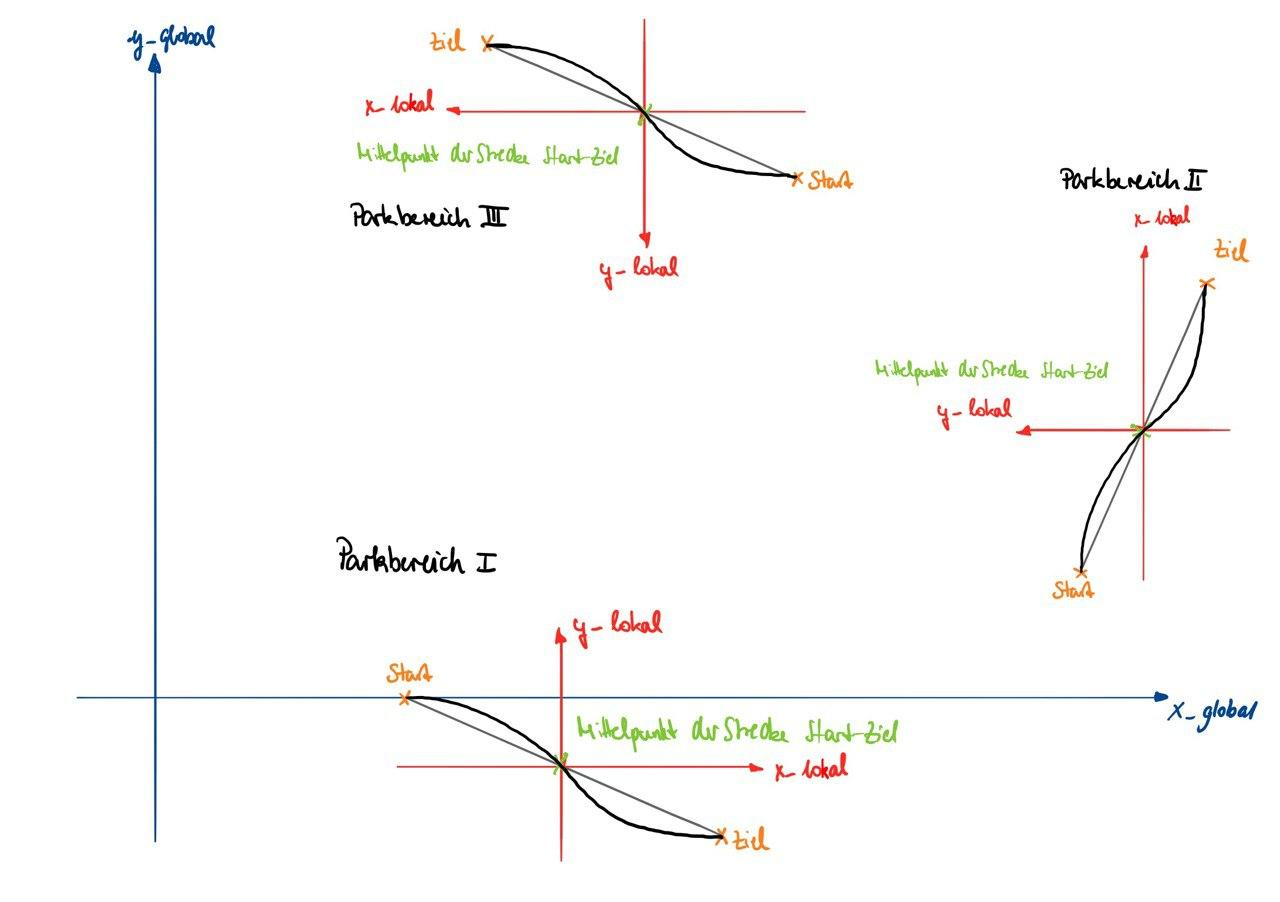
\includegraphics[width=1\textwidth]{SkizzeParklueckenberechung}
	\caption{Skizze für die Parklückenberechung}
	\label{img:grafik-Parkluecke}
\end{figure}